\documentclass{article} % 文書クラスの指定
\usepackage[dvipdfmx]{graphicx}	      %	図を取り込む		   (推奨)
\usepackage{enumitem}                 %	箇条書きを変更する
% \usepackage{caption}                  % caption パッケージの追加
% \captionsetup[figure]{labelsep=} % 図のキャプションの形式を "図6.1(スペース)" に設定
% \captionsetup[table]{labelsep=space}  % 表のキャプションの形式を "表6.1(スペース)" に設定
\usepackage{color}                    % いろいろな色を使えるようにする
\usepackage{url}                      % URLを使えるようにする
\usepackage[left=20mm,right=20mm]{geometry}

% \usepackage{plistings}      % listingsパッケージをpLaTeX上で用いる際の日本語対応処理を強化するためのパッケージ.(plistings.sty)を同一ディレクトリに配置.

\title{音響信号への遅延生成アプリケーション Readme} % 文書のタイトル
\author{知能信号処理研究室\\\\山下一樹} % 著者名
% 所属
\date{\today} % 日付

\begin{document} % 文書の開始
本章では,遅延聴覚フィードバックが身体運動に与える影響の評価方法について述べる.
4章で説明した方法に従い,被験者がボタンを押下する時間を記録すると,被験者に提示するボタンの押下の時間間隔が毎分60回,即ち1000[ms]の間隔でボタンが押下されることが理想である.
しかし,実際には人のボタン押下時間間隔にはばらつきが生じると考えられる.
遅延聴覚フィードバックが身体運動に影響を与える場合,このばらつきは聴覚フィードバックの遅延時間の大きさに応じて変化すると予想される.
そこで,このボタン押下の時間間隔のばらつきを各遅延時間で評価することにより,遅延聴覚フィードバックが身体運動に与える影響を評価する.
ばらつきの評価には,分散と平均二乗誤差を使用し,これらの指標が大きくなるほどばらつきが大きいと判断する.
評価指標を算出する際には,評価指標の値の時間変化や使用するデータの個数が結果に影響を与えるため,
これらをパラメータとして考慮する.
\section{分散}
ボタンを押下する時間間隔の不偏分散$s^2_{a}$は,被験者が行うボタン押下の時間間隔を用いて算出する.$s^2_{a}$は,以下の式により示される.
\begin{equation}
  s^2_a = \frac{1}{l-1} \sum_{i=k}^{k+l-1} (x_i - \bar{x}_{kl})^2
\end{equation}
ここで$l$[回]は分散を算出するために使用するデータの個数,$k$は分析するデータの最初のインデックス,$x_{i}$[ms]は,取得した$i$番目のボタンの押下時間間隔のデータ,$\bar{x}_{kl}$[ms]は,$k$番目のデータから$l$個のデータを用いて算出するボタンの押下時間間隔のデータの平均値を指す.
$s^2_{a}$において,任意の$i$で理想的な時刻にボタンが押下されなかった場合,
$x_{i}$と$x_{i+1}$の両方に理想的なボタンの押下時間間隔との差異が生じる.データの平均値との差異を分析する際,大きな誤差が発生した場合,その影響で分散が過大になり,適切な評価が困難になる可能性がある.
この場合,各被験者のボタンの押下時間間隔のデータの中央値を真値とする分散を検討することが有効である.
中央値を真値として用いることにより,データに極端な誤差が生じた場合でも、ボタンの押下時間間隔のばらつきを適切に評価することが可能になると考えられる.
各被験者のボタンの押下時間間隔のデータの中央値を真値とする分散$s^2_{b}$は,以下の式により示される.
\begin{equation}
  s^2_b = \frac{1}{l} \sum_{i=k}^{k+l-1} (x_i - M_{kl})^2
\end{equation}
ここで,$M_{kl}$は,$k$番目のデータから$l$個のデータを用いて算出するボタンの押下時間間隔のデータの中央値を指す.
次に,真値を理想的なボタンの押下時間間隔とする場合を考える.例えば,ボタン押下の回数が毎分60回であれば,理想的には1000[ms]の間隔でボタンが押下される.
しかし,実際の実験では,この理想的な間隔でボタンが押下されるとは考えにくく,その理想的な間隔との誤差の分散は,
ばらつきが増加するとともに大きくなると推測される.理想的なボタンの押下時間間隔との誤差の分散$s^2_{c}$は,以下の式により示される.
\begin{equation}
  s^2_c = \frac{1}{l} \sum_{i=k}^{k+l-1} (x_i - a)^2
\end{equation}
ここで,$a$は理想的なボタンの押下時間間隔を指す.
% \section{標準偏差}
% まず,ボタンを押下する時間間隔の標準偏差$s_{1}$[ms]は,記録するボタンを押下する時間間隔を用いて算出する.$s_{1}$は次式で表される.
% \begin{equation}
%   s_1 = \sqrt{\frac{1}{n-1} \sum_{i=k}^{k+n-1} (x_i - \bar{x}_{kl})^2}
% \end{equation}
% \begin{equation}
%   s_2 = \sqrt{\frac{1}{n} \sum_{i=k}^{k+n-1} (x_i - M)^2}
% \end{equation}
% \begin{equation}
%   s_3 = \sqrt{\frac{1}{n} \sum_{i=k}^{k+n-1} (x_i - T)^2}
% \end{equation}
\section{平均二乗誤差}
本節では,聴覚フィードバックの遅延が変則的に発生する場合のばらつきの評価について検討する.
ボタンの押下回数が$t$($t$は2以上の整数)の倍数に到達したときのみ遅延が発生する状況を想定し,$t$の倍数に到達する直前のボタン押下時間間隔と直後のボタン押下時間間隔のデータの差の平均二乗誤差(Mean Squared Error, MSE)が,
遅延聴覚フィードバックがボタン押下時間間隔に与える影響を反映すると仮定する.
遅延時間が増加するにつれて,MSEも増加すると予測される.
MSEを算出する際に用いる誤差の総数を表す関数$f(n)$と,使用するデータの最後のインデックスを示す関数$s(n)$は,
ボタンの押下回数$n$を用いて以下の式で表される.

\begin{equation}
f(n) = \left\lfloor \frac{n-t-1}{t} \right\rfloor + 1
\end{equation}
\begin{equation}
s(n) = \left\lfloor \frac{n-t-2}{t-1} \right\rfloor
\end{equation}
ここで,$\left\lfloor x \right\rfloor$は$x$を超えない最大の整数を表す.
これらの関数を用いて,MSEは次の式で定義される.
\begin{equation}
MSE = \frac{1}{f(n)} \sum_{i=0}^{s(n)} (d_{t-1+ti} - d_{t+ti})^2
\end{equation}
ここで,$d_{t-1+ti}$はボタンの押下回数が$t$の倍数に達する直前のボタン押下時間間隔,$d_{t+ti}$はボタンの押下回数が$t$の倍数に達した直後のボタン押下時間間隔のデータを示す.
これにより,聴覚フィードバックの遅延による影響を定量的に評価することが可能になると考えられる.
さらに,$t$の倍数に到達する直前のボタン押下時間間隔と到達した直後の間隔との誤差の中央値(Median Squared Error, MedSE)での評価を検討する.
この計算法により,誤差の中に極端な値が存在しても適切なばらつきの評価が行える可能性がある.
誤差の中央値MedSEは以下の式で定義される.
\begin{equation}
MedSE = Med\left((d_{t-1}-d_{t})^2, (d_{2t-1}-d_{2t})^2, \ldots, (d_{(1+s(n))t-1}-d_{(1+s(n))t})^2\right) \label{eq:MedSE}
\end{equation}
式\ref{eq:MedSE}における$Med()$は中央値を計算する関数であり,
括弧内の各項はボタンの押下回数が$t$の倍数に到達する直前のボタン押下時間間隔と$t$の倍数に到達した直後のボタン押下時間間隔の差の二乗を表す.
このように,MedSEを用いることで,データの極端なばらつきがあった場合でも,
遅延聴覚フィードバックがボタン押下時間間隔に与える影響を適切に評価することが可能になると考えられる.

% \section{絶対値誤差}


% \maketitle % タイトル、著者名、日付の表示
% 本稿は、客観調査のためのアプリケーションを使用するための説明書である。
% \section{各要素の説明} 
% 図\ref{fig:app_kyakkann}にアプリケーションの画面を示す。
% 以下に赤色の点線で囲った各要素について説明する。
% \begin{figure}[tbp]
%   \centering
%   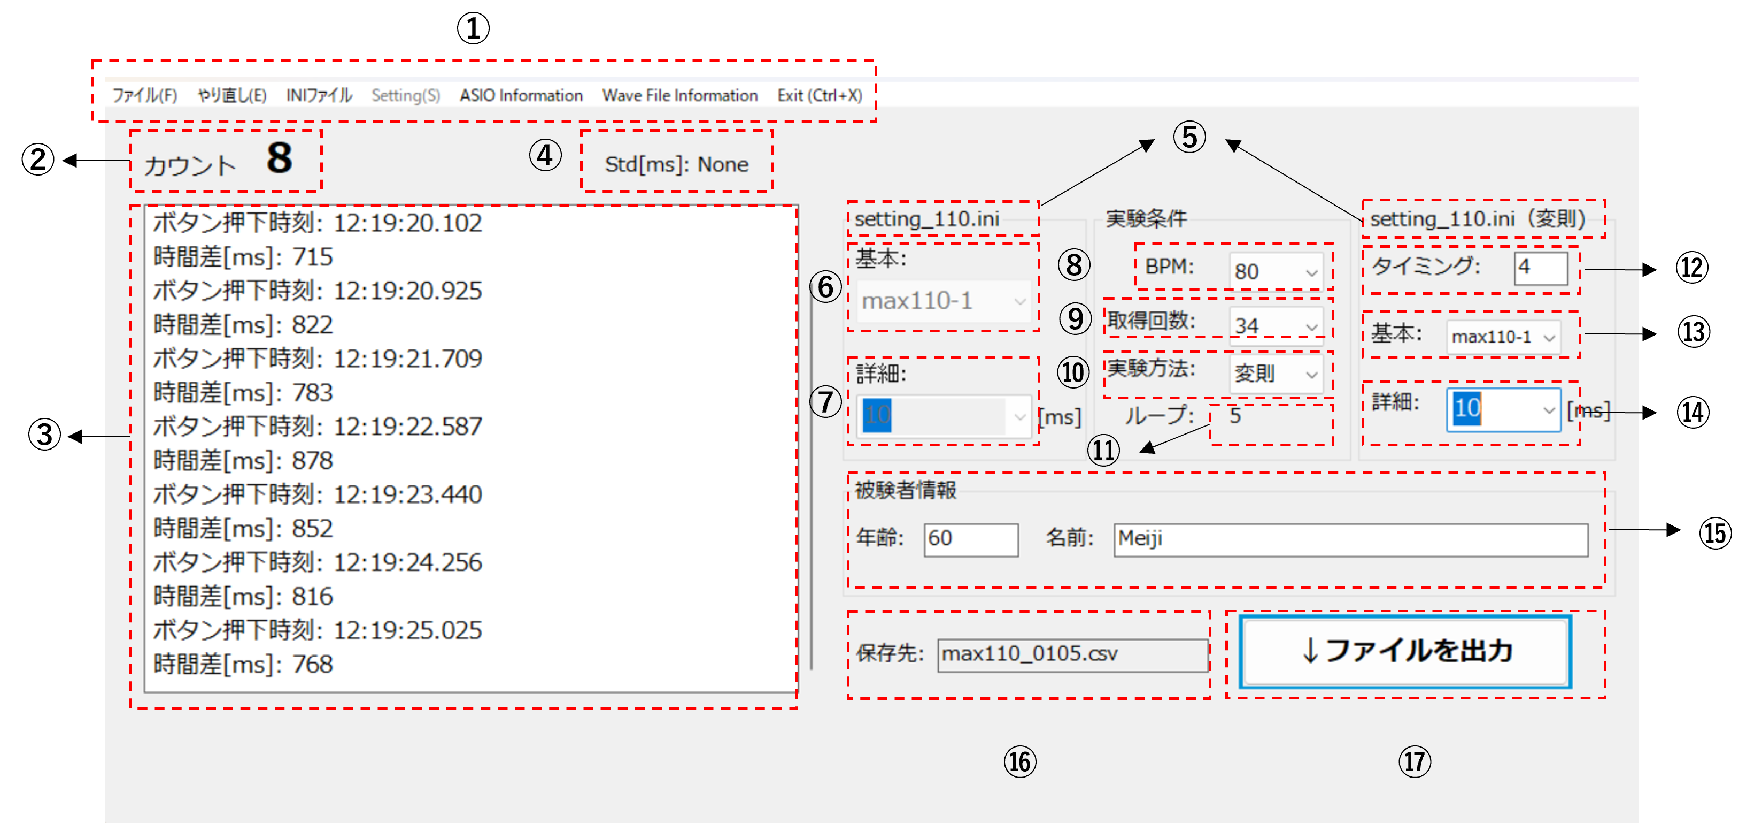
\includegraphics[scale=0.5]{figures_app_1.pdf}
%   \caption{アプリケーションの画面}
%   \label{fig:app_kyakkann}
% \end{figure}
% \begin{enumerate}
%   \item メニューバー。アプリケーションの操作に関するメニューが表示される。
%   「ファイル」は、結果を保存するためのCSVファイルを選択するためのメニューである。
%   「やり直し」は、ボタンの押下回数をリセットするためのメニューである。
%   「INIファイル」は、遅延時間が記述されているiniファイルを選択するメニューである。このiniファイルは指定されたフォルダ内に保存されていなければならない。詳細は2章を参照。
%   \item ボタンの押下回数を表示する。
%   \item ボタンの押下時刻と前回押した時刻のとの差[ms]を表示する。 
%   \item ボタンの押下時間間隔[ms]のデータの標準偏差を表示する。外れ値を含むすべてのデータの標準偏差を表示する。
%   分析データとしてはこの値は使用しない。
%   \item 設定したiniファイル名を表示する。
%   \item 指定したiniファイルに記述された遅延時間のグループ名を表示するコンボボックス。
%   \item (6)で選択された遅延時間のグループ名の遅延時間[ms]を表示するコンボボックス。
%   \item CSVファイルに出力するBPMの値を指定するためのコンボボックス。デフォルトは80。
%   \item ボタンの押下時間間隔の取得回数を指定するためのコンボボックス。デフォルトは34。(2)がここで指定した回数に到達すると、
%   メッセージボックスが出力され音の出力が一時的に停止する。
%   \item 実験方法を指定するためのコンボボックス。デフォルトは「変則」。
%   変則に設定すると、右側のコンボボックスが有効化される。通常の場合、(7)で設定した遅延時間で音が毎回出力される。
%   変則の場合、(12)で指定した倍数に到達すると音声に遅延が(14)で指定した遅延時間だけ加えられる。それ以外の場合は、(7)で指定した遅延時間だけ加えられた音声が出力される。
%   \item プログラム中で設定するfor分のループ回数。この値が小さい程遅延時間が小さい。アプリ開発中に使用していたため、現在は使用していない。
%   \item 遅延のタイミングを指定するためのエディットボックス。デフォルトは4。ここで指定された値の倍数に(2)が到達すると音声に遅延が(14)で指定した遅延時間だけ加えられる。
%   \item (1)で設定したiniファイルのグループ名を指定するためのコンボボックス。
%   \item (13)で指定したグループの遅延時間[ms]を指定するためのコンボボックス。
%   \item 被験者の情報を入力するためのエディットボックス。ここに書かれた情報もCSVファイルに書き込まれる。
%   後続のデータ分析などに利用される。
%   \item (1)で選択したCSVファイルの名前を表示する。
%   \item 結果を保存するためのプッシュボタン。押下すると、(1)で指定したファイル名でCSVファイルが保存される。(10)で指定した実験方法により、書き込むデータの内容が若干異なる。
% \end{enumerate}

% \section{INIファイルの設定}
% アプリケーションがiniファイルに記述された遅延時間を読み込むために、exeファイルと同じフォルダ内に、
% 「setting」という名前のフォルダを作成し、その中に遅延時間を記述したiniファイルを保存する必要があります。
% setting\_110.iniファイルに遅延時間を設定して置くことができます。iniファイルはテキストエディタで編集可能です。
% 以下にiniファイルの例を示します。
% まず、「setting」セクション内の「latedataname」キーに遅延時間のグループ名を設定します。
% 次に、設定した遅延時間のグループ名のセクションを作成し、「data」キーにカンマ区切りで遅延時間を設定します。
% これを行うとアプリケーションで遅延時間を読み込むことができます。
% \begin{figure}[tbp]
%   \centering
%   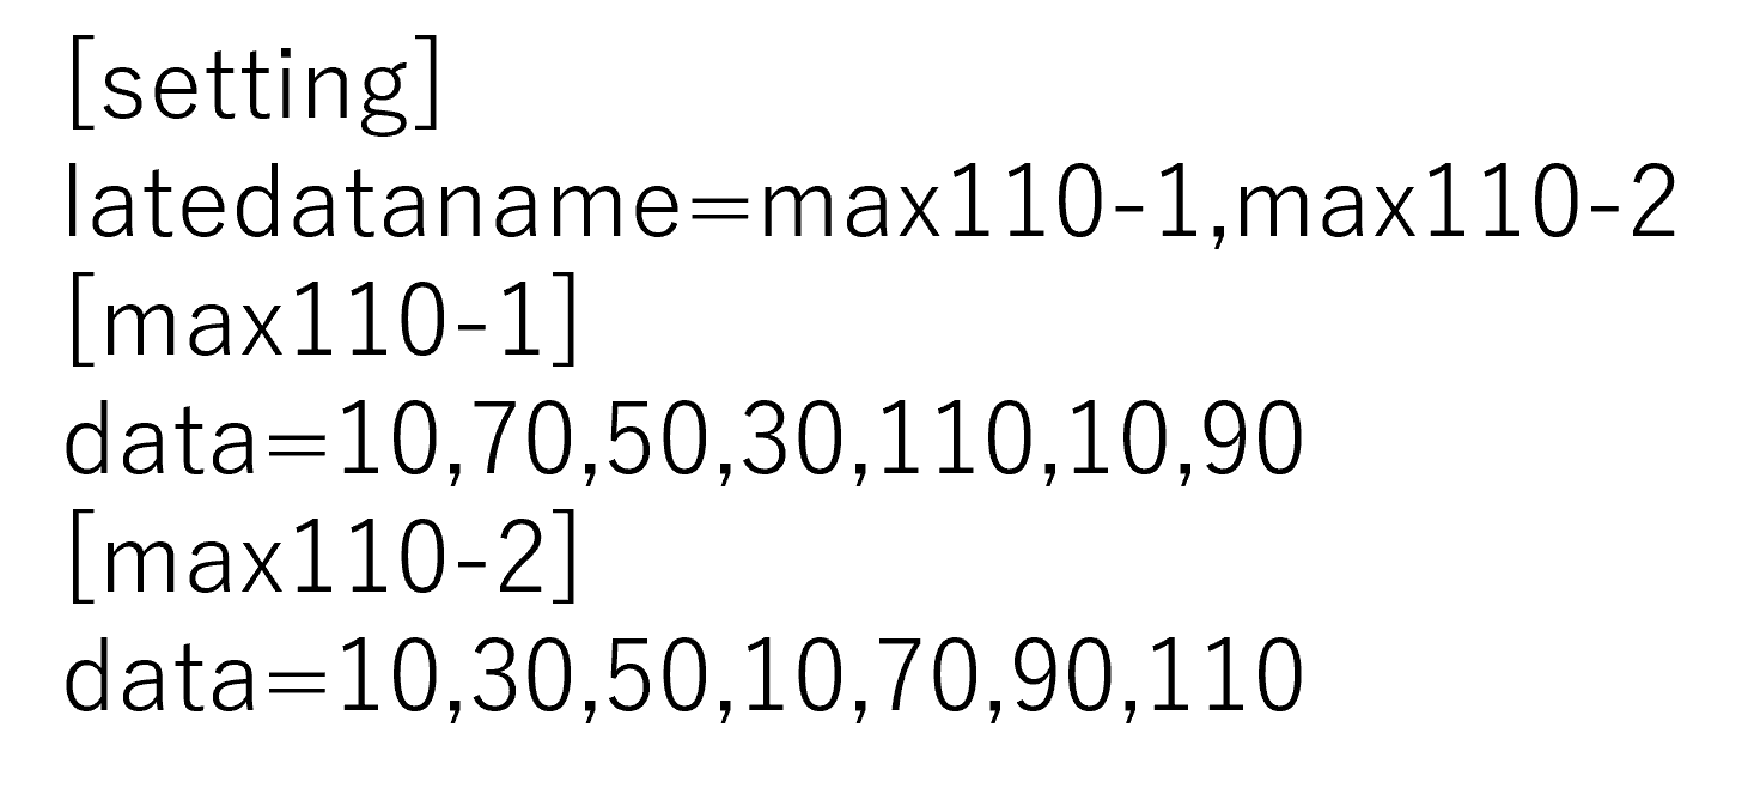
\includegraphics[scale=0.3]{setting-ini.pdf}
%   \caption{setting.iniの例}
%   \label{fig:ini-file}
% \end{figure}

% \section{改善点}
% \begin{enumerate}
%   \item iniファイルのデフォルト名が「setting\_110.ini」になっている。そのため、決まったフォルダ内に「setting\_110.ini」が保存されていなければならない。
%   \item 音声の出力先のチャンネル数を指定できるようにする。
%   \item ボタンの押下回数が指定された回数に到達したときに、メッセージボックスによって強制的に音声の出力を一時的に停止する機能があるが、
%   メッセージボックスを閉じた直後に音声が出力されないようにしたい。
% \end{enumerate}
\end{document} % 文書の終了
